% ==========================================================================
% GENERATED FILE (v3 build). Assembled by ../deck_support/scripts/assemble_deck.py
% from ../deck_support/redesign/preamble_madrid.tex, redesign/v3/W1-W5_frames.tex,
% backups_old.tex, backups_old2.tex and backups_new.tex; checked by scripts/lint_deck.py and
% scripts/layout_sim/v3_fit.py. Edit the sources and re-run, or port any
% Overleaf edit back to the sources before the next assembly.
% ==========================================================================
% ==========================================================================
% The Price of Flexibility -- MOM Tripartite Meeting, January 2027
% SMU x SNEF study on flexible work arrangements (FWAs) for PMEs
%
% Look: Madrid theme as in the PI's BOK Pohang talk (myblue / myred), with the
% polish pass of 7 Oct 2026 (reviews/claude_round5/DESIGN_PLAN.md s1.1): one
% type family (Helvetica, as the figures' Arial), centred content blocks,
% one card, table, note and button grammar for every slide.
% Build: pdfLaTeX on Overleaf; compile twice (hyperlinks, page totals).
% Upload to the Overleaf project root: this main.tex and the folders
% figures/ and tables/ (generated by ../deck_support/scripts/).
%
% Every number on a slide is traced to ../deck_support/EVIDENCE_BOOK.md;
% fact IDs (e.g. [E3], [Q5]) are given in comments beside the numbers.
% Speaker notes: \note{} after each main slide (timed script in
% ../deck_support/SPEAKER_SCRIPT.md). To show notes on a second screen,
% uncomment the two NOTES lines below (test the backup links in that build).
%
% Frame rule (polish pass): every frame body starts with \FrameTop (except
% M-title, M-thanks, B-index and B-index-all). It centres the content block
% between the title bar and the note/button row, and, being a control
% sequence, it stops beamer from reading a leading {...} group as a frame
% subtitle (the cause of the black-on-blue slides 7 and 19). A non-empty
% subtitle now stops the compile with an error.
% ==========================================================================
\documentclass[aspectratio=169,11pt]{beamer}

% \usepackage{pgfpages}                                   % NOTES
% \setbeameroption{show notes on second screen=right}     % NOTES

\usetheme{Madrid}
\usecolortheme{default}
\setbeamertemplate{navigation symbols}{}
\setbeamersize{text margin left=0.6cm,text margin right=0.6cm}   % text width 14.8 cm (all figures and tables are sized to it)

\usepackage[T1]{fontenc}
\usepackage[utf8]{inputenc}
\usepackage{lmodern}                 % kept for math symbols
\usepackage[scaled=0.92]{helvet}     % G1: one type family; Helvetica matches the figures' Arial
\renewcommand{\familydefault}{\sfdefault}
\usepackage{graphicx}
\usepackage{booktabs}
\usepackage{tabularx}
\usepackage{array}
\usepackage{multirow}
\usepackage{amsmath}
\usepackage{amssymb}
\usepackage{ragged2e}
\usepackage{tikz}
\usetikzlibrary{positioning,calc,arrows.meta}
\usepackage{appendixnumberbeamer}

\graphicspath{{figures/}{./}}

% No hyphenation on slides: a word or a range (1--2, 17--33) never breaks.
\hyphenpenalty=10000 \exhyphenpenalty=10000
\setlength{\emergencystretch}{2em}   % without hyphenation, a ragged line may run long; loosen instead

% Guards: if a stray Unicode symbol slips into the source, typeset it
% (declared by code point, so this preamble itself stays ASCII-only).
\ifdefined\DeclareUnicodeCharacter % pdfLaTeX (Overleaf); XeTeX reads Unicode natively
\DeclareUnicodeCharacter{2248}{\ensuremath{\approx}}
\DeclareUnicodeCharacter{2264}{\ensuremath{\le}}
\DeclareUnicodeCharacter{2265}{\ensuremath{\ge}}
\DeclareUnicodeCharacter{2192}{\ensuremath{\rightarrow}}
\DeclareUnicodeCharacter{2212}{\ensuremath{-}}
\fi

% --------------------------------------------------------------------------
% Colours: the PI's palette (BOK talk). No pastel tints.
% Navy is structure only (title bar, banner, accent bars, bullets, links);
% neutral labels are Ink.
% --------------------------------------------------------------------------
\definecolor{myblue}{RGB}{0,51,102}
\definecolor{myred}{RGB}{153,0,0}
\setbeamercolor{structure}{fg=myblue}
\setbeamercolor{alerted text}{fg=myred}
% Semantic names used throughout the frames
\colorlet{Navy}{myblue}
\colorlet{Employee}{myblue}        % PMEs
\colorlet{Employer}{myred}         % employers
\definecolor{Ink}{HTML}{1A1A1A}
\definecolor{Muted}{HTML}{555555}
\definecolor{Rule}{HTML}{A6A6A6}
\definecolor{Soft}{HTML}{EBEBEB}   % neutral light grey (no tint); F2F2F2 washed out on a projector
\colorlet{SoftBlue}{Soft}
\colorlet{SoftCopper}{Soft}
% Every slide uses the same white canvas and the same box colours (PI, 6 Oct
% 2026). Set explicitly so nothing depends on how Madrid and the default
% colour theme combine.
\setbeamercolor{normal text}{fg=Ink,bg=white}
\setbeamercolor{background canvas}{bg=white}
\setbeamertemplate{background canvas}[default]
\setbeamercolor{frametitle}{fg=white,bg=myblue}

% --------------------------------------------------------------------------
% Type scale (G1). helvet is scaled 0.92, so nominal 11.5 / 10.5 / 9.5 print
% close to the figures' Arial 10.5 / 9.5 / 9. Only these sizes in W1-W5.
% --------------------------------------------------------------------------
\newcommand{\FsHead}{\fontsize{11.5}{14}\selectfont\bfseries}   % card/zone headings, question line
\newcommand{\FsBody}{\fontsize{10.5}{12.8}\selectfont}          % card bodies, cells, \Interp
\newcommand{\FsSmall}{\fontsize{10}{12}\selectfont}             % secondary lines, chips, dense cells
\newcommand{\FsTable}{\fontsize{10}{12.2}\selectfont}           % main tables
\newcommand{\FsTableTight}{\fontsize{9.5}{11.6}\selectfont}     % M-options only (table under the banner)
% Final fixer (7 Oct 2026, visual QA): 7.5 pt x 0.92 printed at 6.9 pt, under the 8 pt floor, and the polish
% pass moved figure caveats (what * and grey mean, filled/hollow, the 198 contrasts) into this block; 8.7 pt
% x 0.92 prints at 8.0 pt, the figures' FS_NOTE floor.
\newcommand{\FsNote}{\fontsize{8.7}{9.8}\selectfont}             % note/source block (prints at 8.0 pt)
\setbeamerfont{itemize/enumerate body}{size=\fontsize{10.5}{13}\selectfont}
\setbeamerfont{itemize/enumerate subbody}{size=\fontsize{9.5}{12}\selectfont}

% --------------------------------------------------------------------------
% Frame title (G3): bold, one line, text on the 0.6 cm text margin, navy bar
% 0.98 cm tall as before. A non-empty subtitle is an error: it means a frame
% body was read as a subtitle (put \FrameTop first in the body).
% --------------------------------------------------------------------------
\setbeamerfont{frametitle}{size=\fontsize{14.4}{17.3}\selectfont,series=\bfseries}
\makeatletter
\setbeamertemplate{frametitle}{%
  \ifx\insertframesubtitle\@empty\else
    \PackageError{deck}{Frame body read as a frame subtitle}{Put \string\FrameTop\space first in the frame body}\fi
  \nointerlineskip
  \begin{beamercolorbox}[wd=\paperwidth,ht=0.64cm,dp=0.34cm,leftskip=0.6cm,rightskip=0.6cm]{frametitle}%
    \usebeamerfont{frametitle}\insertframetitle
  \end{beamercolorbox}}
\makeatother

% --------------------------------------------------------------------------
% Title page (G4): no box, no shadow; centred hierarchy of title, subtitle,
% rule, author, affiliation, the SNEF joint-work line (\JointWork, from W1)
% and the date line.
% --------------------------------------------------------------------------
\setbeamertemplate{title page}{%
  \centering
  {\color{Navy}\fontsize{24}{28.8}\selectfont\bfseries\inserttitle\par}\vspace{0.25cm}
  {\color{Ink}\fontsize{13}{16}\selectfont\insertsubtitle\par}\vspace{0.40cm}
  {\color{Navy}\rule{3cm}{0.8pt}\par}\vspace{0.40cm}
  {\color{Ink}\fontsize{12}{14.4}\selectfont\bfseries\insertauthor\par}\vspace{0.10cm}
  {\color{Ink}\FsBody\insertinstitute\par}\vspace{0.06cm}
  {\color{Muted}\FsBody\JointWork\par}\vspace{0.50cm}
  {\color{Muted}\fontsize{9.5}{11.4}\selectfont\insertdate\par}}

% --------------------------------------------------------------------------
% Inner theme: flat bullets, plain bold numerals, flat blocks (no rounded
% corners, no shadow). Blocks: Soft fill, Navy heading, Navy top accent.
% --------------------------------------------------------------------------
\setbeamertemplate{itemize items}[circle]
\setbeamertemplate{itemize subitem}[circle]
\setbeamercolor{itemize item}{fg=Navy}
\setbeamercolor{itemize subitem}{fg=Navy}
\setbeamertemplate{enumerate items}[default]
\setbeamerfont{enumerate item}{series=\bfseries}
\setbeamercolor{enumerate item}{fg=Navy}
\setbeamertemplate{blocks}[default]
\setbeamercolor{block title}{fg=Navy,bg=Soft}
\setbeamercolor{block title alerted}{fg=Navy,bg=Soft}
\setbeamercolor{block body}{fg=Ink,bg=Soft}
\setbeamercolor{block body alerted}{fg=Ink,bg=Soft}
\setbeamerfont{block title}{size=\fontsize{11.5}{14}\selectfont,series=\bfseries}
\setbeamerfont{block title alerted}{size=\fontsize{11.5}{14}\selectfont,series=\bfseries}
\setbeamertemplate{block alerted begin}{%
  \par\vskip\medskipamount
  {\color{Navy}\hrule height 0.07cm}\nointerlineskip
  \begin{beamercolorbox}[wd=\textwidth,leftskip=0.25cm,rightskip=0.25cm,ht=0.62cm,dp=0.18cm]{block title alerted}%
    \usebeamerfont*{block title alerted}\insertblocktitle
  \end{beamercolorbox}%
  {\parskip0pt\par}\nointerlineskip
  \usebeamerfont{block body alerted}%
  \begin{beamercolorbox}[wd=\textwidth,leftskip=0.25cm,rightskip=0.25cm,vmode]{block body alerted}%
    \vskip0.02cm}
\setbeamertemplate{block alerted end}{\vskip0.20cm\end{beamercolorbox}\vskip\smallskipamount}

% --------------------------------------------------------------------------
% Navigation buttons (G9): small, muted outline pills
% --------------------------------------------------------------------------
\setbeamercolor{button}{bg=white,fg=Muted}
\setbeamercolor{button border}{fg=Rule}
\setbeamerfont{button}{size=\fontsize{7}{8.4}\selectfont}

% --------------------------------------------------------------------------
% Footer: frame number only (as in the BOK talk); "Backup B<n>" in backups
% --------------------------------------------------------------------------
\setbeamerfont{page number in head/foot}{size=\fontsize{7}{8.4}\selectfont}
\setbeamercolor{page number in head/foot}{fg=Muted}
\newif\ifinbackup
\inbackupfalse
\setbeamertemplate{footline}{%
  \leavevmode\hbox{%
  \begin{beamercolorbox}[wd=\paperwidth,ht=0.30cm,dp=0.14cm,leftskip=0.6cm,rightskip=0.6cm]{}%
    \usebeamercolor[fg]{page number in head/foot}\usebeamerfont{page number in head/foot}%
    \ifinbackup\hyperlink{B-index}{\textcolor{myblue}{Backup index}}\fi
    \hfill
    \ifinbackup Backup B\insertframenumber\else\insertframenumber\,/\,\inserttotalframenumber\fi
  \end{beamercolorbox}}}

% --------------------------------------------------------------------------
% Booktabs (G8): one table style
% --------------------------------------------------------------------------
\setlength{\heavyrulewidth}{0.8pt}
\setlength{\lightrulewidth}{0.4pt}
% Final fixer: 0.08 cm under the bottom rule, so an \Interp line under a main table has the air it has under a
% figure (a figure carries its own white margin; \Interp itself now adds only 0.06 cm).
\newcommand{\MainTableStyle}{\FsTable\setlength{\tabcolsep}{4pt}\renewcommand{\arraystretch}{1.15}%
  \setlength{\belowbottomsep}{0.08cm}}
\newcommand{\RowSep}{\addlinespace[3pt]}
\newcommand{\HeadB}[2]{\parbox[b]{#1}{\raggedright\bfseries #2}}   % bottom-aligned bold header cell

% --------------------------------------------------------------------------
% Cards (G7): one shared TikZ style for every card, cell, chip and arrow
%   \DeckCard{x0}{y0}{x1}{y1}{accent}: Soft card with a 0.07 cm top accent bar
%   (myblue for PME or neutral cards, myred for employer cards).
%   deckheld (dashed) is reserved for "held constant / applies to all".
% --------------------------------------------------------------------------
\tikzset{
  deckcard/.style={fill=Soft,draw=none},
  deckhead/.style={anchor=north west,inner sep=0pt,align=flush left,font=\FsHead,text=#1},
  deckhead/.default=Navy,
  deckbody/.style={anchor=north west,inner sep=0pt,align=flush left,font=\FsBody,text=Ink},
  deckcell/.style={fill=Soft,draw=none,inner xsep=0.08cm,inner ysep=0.03cm,align=center,font=\FsBody,text=Ink},
  deckheld/.style={fill=white,draw=Rule,dashed,line width=0.4pt,align=center,font=\FsSmall,text=Muted},
  deckchip/.style={fill=Soft,draw=none,minimum height=0.55cm,inner xsep=0.12cm,align=center,font=\FsSmall,text=Ink},
  deckdisc/.style={circle,fill=Ink,text=white,inner sep=0pt,minimum size=0.55cm,font=\fontsize{11}{13}\selectfont\bfseries},
  deckcolhead/.style={anchor=base west,inner sep=0pt,font=\FsBody\bfseries},
  deckarrow/.style={-{Stealth[length=1.6mm]},draw=Muted,line width=0.8pt}}
\newcommand{\DeckCard}[5]{\fill[deckcard] (#1,#2) rectangle (#3,#4); \fill[#5] (#1,#2) rectangle (#3,#2-0.07);}

% --------------------------------------------------------------------------
% Text elements (API used by the frames)
% --------------------------------------------------------------------------
\newcommand{\ap}{\ensuremath{\approx}\,}
\newcommand{\dg}{\textsuperscript{\textdagger}}
\newcommand{\DgNote}{\textsuperscript{\textdagger}Range across two samples: all respondents, and excluding one online panel with less reliable survey answers.}
\newcommand{\DgShort}{\textsuperscript{\textdagger}Range across all respondents and excluding one online panel.}
\newcommand{\TableFont}{\fontsize{8.5}{10}\selectfont}
\newcommand{\Caveat}[1]{\par{\color{Ink}\fontsize{10}{12}\selectfont\bfseries #1\par}\vspace{0.06cm}}

% Implication / key message box. Not used on any slide (no implication boxes);
% kept so an old source line still compiles.
\newcommand{\Takeaway}[1]{%
  \par\vspace{0.04cm}%
  \begin{alertblock}{\fontsize{9.5}{11.4}\selectfont #1}\end{alertblock}}

\newcommand{\PanelTitle}[2]{\par{\color{#1}\fontsize{10}{12}\selectfont\bfseries #2\par}\vspace{0.04cm}}
\newcommand{\BigStat}[3]{%
  {\color{#1}\fontsize{15}{17}\selectfont\bfseries #2\par}%
  {\color{Ink}\fontsize{8.5}{10}\selectfont\RaggedRight #3\par}\vspace{0.06cm}}
\newcommand{\Body}[1]{{\fontsize{9.5}{11.6}\selectfont\RaggedRight #1\par}}

% --------------------------------------------------------------------------
% Vertical balance and the frame ending (G2, G6, G9)
%   \FrameTop          first token of every frame body: stretch above the content
%   body / figure -> \Interp -> \SourceNote -> \Backups (or \BackTo, \BackToTwo)
% The content block is centred between the title bar and the note/button rows:
% \FrameTop and the glue before the note block (or, without a note, before the
% buttons) share the free space. The note block sits on the row just above the
% buttons, which sit on the last row above the footer (PI directive 8).
% Every \SourceNote is followed by \Backups, \BackTo or \BackToTwo in the same
% frame (lint_deck.py checks this).
% --------------------------------------------------------------------------
% \FrameTop takes back 0.15 cm of beamer's fixed 0.2 cm [t] top skip, so the block
% sits optically centred (measured: equal stretch alone left the top gap 0.27 cm
% larger than the bottom gap on every slide).
\newif\ifdeckSrc
\newcommand{\FrameTop}{\global\deckSrcfalse\vskip -0.15cm plus 1filll\relax}
% Final fixer (7 Oct 2026): at 8.0 pt most notes run to 2 lines. To make room, the button row is set on the
% button font's own leading (\DeckBtnRow: the buttons stay on the same last row; only the dead glue above
% them goes), \Interp sits 0.06 cm under the figure (was 0.15), and the note keeps a fixed 0.06 cm from the
% text above it, so it never touches the \Interp lines on a full slide. The note is \raggedright (not
% ragged2e's \RaggedRight, whose 2em stretch let an unbreakable 'Benjamini--Hochberg' overrun the line).
\newcommand{\SourceNote}[1]{\par\vskip 0.06cm plus 1filll\relax
  {\color{Muted}\FsNote\raggedright #1\par}\vspace{0.12cm}\global\deckSrctrue}
\newcommand{\DeckNavGlue}{\par\ifdeckSrc\else\vskip 0pt plus 1filll\relax\fi\global\deckSrcfalse}
\newcommand{\Interp}[1]{\par\vspace{0.06cm}{\centering\color{Ink}\FsBody #1\par}}
\newcommand{\BL}[2]{\hyperlink{#1}{\beamergotobutton{#2}}\hspace{0.15cm}\ignorespaces}
\newcommand{\DeckBtnRow}{\usebeamerfont{button}\baselineskip=8.4pt\relax}
\newcommand{\Backups}[1]{\DeckNavGlue{\DeckBtnRow\noindent\hfill#1\unskip\par}}
% Return links. In the short build (main_short.tex) a backup may point back to
% a main slide that the short path omits; the link then goes to the backup
% index instead, so every link resolves in both builds. The footer carries
% the "Backup index" link on every backup.
\makeatletter
\providecommand{\ShortLabels}{}
\newcommand{\bt@target}{}
\newcommand{\bt@set}[1]{%
  \ifdefined\ShortPath
    \@expandtwoargs\in@{,#1,}{,\ShortLabels,}%
    \ifin@\def\bt@target{#1}\else\def\bt@target{B-index}\fi
  \else\def\bt@target{#1}\fi}
\newcommand{\BackTo}[2]{%
  \DeckNavGlue{\DeckBtnRow\noindent\hfill
  \bt@set{#1}\hyperlink{\bt@target}{\beamerreturnbutton{#2}}\par}}
\newcommand{\BackToTwo}[4]{%
  \DeckNavGlue{\DeckBtnRow\noindent\hfill
  \bt@set{#1}\hyperlink{\bt@target}{\beamerreturnbutton{#2}}%
  \hspace{0.15cm}\bt@set{#3}\hyperlink{\bt@target}{\beamerreturnbutton{#4}}\par}}
\makeatother
\AtBeginEnvironment{frame}{\global\deckSrcfalse}
\newcommand{\BI}[2]{\hyperlink{#1}{\textcolor{myblue}{#2}}\par}
\newcommand{\BIi}[2]{\hyperlink{#1}{\textcolor{myblue}{#2}}}
\newcommand{\BH}[1]{\vspace{0.12cm}{\color{Ink}\fontsize{9.5}{11.4}\selectfont\bfseries #1\par}}

% Employer update (appended sample, n = 397; appended_clogit.xlsx / appended_wtp.xlsx, 9 Oct 2026):
% \Pend marks an employer value that the appended_* outputs do not contain, so the old 303-firm value is
% kept and shown in red until it is re-estimated. To print them normally: \renewcommand{\Pend}[1]{#1}.
\newcommand{\Pend}[1]{\textcolor{red}{#1}}
\newcommand{\Fig}[2]{{\centering\includegraphics[width=\linewidth,height=#2,keepaspectratio]{#1}\par}}
% Round 5 result-slide grammar (PI directive 7): one large centred figure drawn
% at true size (13.0 x 5.0 cm unless stated), one or two short interpretation
% lines, the note/source block, then the button row.
\newcommand{\FigC}[1]{{\centering\includegraphics{#1}\par}}
% Decision banner (M-options, M-conclusion): navy box, white bold text
\setbeamercolor{decision}{fg=white,bg=myblue}
\newcommand{\DecisionBanner}[1]{\par
  \begin{beamercolorbox}[wd=\textwidth,sep=0.10cm,center,rounded=false]{decision}%
    {\fontsize{10.5}{12.6}\selectfont\bfseries #1}\end{beamercolorbox}\par}

\newcommand{\Tab}[1]{{\centering\TableFont\input{tables/#1}\par}}
\newcommand{\BackupFig}[7]{%
  \begin{frame}[t,label=#1]{#2}
    \FrameTop
    \Fig{#3}{#4}
    \SourceNote{#7}
    \BackTo{#5}{#6}
  \end{frame}}
\newcommand{\BackupTab}[6]{%
  \begin{frame}[t,label=#1]{#2}
    \FrameTop
    \Tab{#3}
    \SourceNote{#6}
    \BackTo{#4}{#5}
  \end{frame}}

\title[The Price of Flexibility]{The Price of Flexibility}
\subtitle{What PMEs value, what employers weigh, and where they meet}
\author[Seonghoon Kim]{Seonghoon Kim}
\institute[SMU]{Singapore Management University}
\newcommand{\JointWork}{Joint work with the Singapore National Employers Federation (SNEF)}
\date[January 2027]{Preliminary findings for tripartite discussion \textbar\ January 2027}
\hypersetup{pdftitle={The Price of Flexibility},pdfauthor={Seonghoon Kim},
  pdfsubject={Flexible work arrangements in Singapore: PMEs and employers},
  pdfkeywords={flexible work arrangements; TG-FWAR; choice experiment; PMEs; employers}}

% Option backups (B-optA-D): label, title, zone line, evidence, who could act,
% builds on, not, watch, closing code (source note and return buttons)
\newcommand{\OptionFrame}[9]{%
  \begin{frame}[t,label=#1]{#2}
    \FrameTop % first body token (centring; never a frame subtitle)
  % polish pass (BKb): the zone line is a neutral Ink meta line over a hairline Rule;
  % Navy stays for the panel headings (structure); 0.12 cm between panels. After the
  % rule, prevdepth 0 restores the baseline skip that the T-aligned columns need.
  {\fontsize{9}{11}\selectfont
    \noindent{\color{Ink}#3}\par
    \vspace{0.06cm}{\color{Rule}\hrule height 0.4pt}\prevdepth=0pt
    \begin{columns}[T,onlytextwidth]
      \begin{column}{0.54\textwidth}
        \PanelTitle{Navy}{The evidence}
        #4\par
        \vspace{0.12cm}
        \PanelTitle{Navy}{Owner and first step}
        #5\par
      \end{column}
      \begin{column}{0.42\textwidth}
        \PanelTitle{Navy}{Builds on}
        #6\par
        \vspace{0.12cm}
        \PanelTitle{Navy}{What it is not}
        #7\par
        \vspace{0.12cm}
        \PanelTitle{Navy}{What to watch}
        #8\par
      \end{column}
    \end{columns}\par}
    #9
  \end{frame}}

% Short presentation build (round 5): compile main_short.tex for the 15-frame
% path below plus every backup; return links to omitted main slides go to the index.
\def\ShortLabels{M-title,M-motivation,M-question,M-framework,M-design,M-pmes,M-why-pmes,M-employers,M-where,M-meet,M-puzzle,M-barriers,M-options,M-conclusion,M-thanks}
\ifdefined\ShortPath
  \includeonlyframes{M-title,M-motivation,M-question,M-framework,M-design,M-pmes,M-why-pmes,M-employers,M-where,M-meet,M-puzzle,M-barriers,M-options,M-conclusion,M-thanks,B-index,B-index-all,B-laboursupply,B-talent,B-triangulation,B-guidelines,B-partners,B-legal,B-intl,B-zones,B-validity,B-sample,B-industry,B-panel,B-governance,B-cards,B-paygaps,B-hedonic,B-methods,B-eqpay,B-landscape,B-setup,B-emp-all,B-remote-commute,B-emp-benchmarks,B-why-pmes,B-emp-groups,B-access,B-emp-robust,B-org-yardstick,B-org-salary,B-why-org,B-org-splits,B-org-concerns,B-org-view,B-industry-note,B-modelfree,B-puzzle,B-pilot,B-flexiload,B-career-who,B-career,B-tgfwar,B-awareness,B-approvals,B-approvals-tab,B-requestrate,B-limits,B-nextsteps,B-followup,B-optA,B-optB,B-optC,B-optD,B-optD-items,B-why-org-tests,B-language,B-org-pct,B-gap,B-ra-gender,B-ra-age,B-ra-care,B-ra-role,B-ra-edu,B-ra-sameside,B-ra-trim}
\fi

\begin{document}

% ##########################################################################
% Main slides from redesign/v3/W1_frames.tex
% ##########################################################################
\begin{frame}[plain,label=M-title]
  \titlepage
\end{frame}
% Note numbers: [S1] 1,020 PMEs; [S2] 397 people involved in PME hiring or manpower decisions; [S5, S6] mirrored choices on a common menu
% Removed from the round-4 note, pending the PI: "the analysis and options are the SMU team's" - a governance fact, see B-governance
\note{[Short path] Colleagues from MOM, NTUC and SNEF: the question for Singapore is no longer whether flexible work exists, but which arrangements can retain PMEs while remaining workable for firms.
In this joint study with SNEF, 1,020 PMEs and 397 people involved in PME hiring or manpower decisions made mirrored choices on a common menu of arrangements. % [S1, S2, S5]
The results point to common ground, a role-dependent case, and arrangements that need testing before scaling.
Values in per cent of pay are a measuring rod, not a proposal to lower pay.
The findings are preliminary; we end with a decision for the partners.
[Timing: 130 words a minute plus 15 seconds a slide. Short path, 15 slides, target 17 to 18 minutes: Title, Motivation, Question, Framework, Design, PMEs, Why PMEs, Employers, Where, Meet, Compressed week, Barriers, Options, Conclusion, Thank you. The full deck adds Literature, Data, Estimation, Descriptive, Groups, Robustness, Discussion and Limits.]}

% ==========================================================================
% 2. MOTIVATION   [short path]
% ==========================================================================
% Directive 1: the figure is large, centred and dominant (F_motivation drawn at true size 14.0 x 5.0 cm, FigC).
% Directive 3: the mandated title and caption state the policy problem, fit; no bullet column.
\begin{frame}[t,label=M-motivation]{Flexible work is mainstream; the policy problem is fit}
  % F_motivation: establishments with 25+ staff, private plus the public sector, offering at least one scheduled
  % FWA, June 2008-2025 [P4s, P4]; title "Establishments (25+ staff, incl. public sector)", fixer pass 7 Oct 2026;
  % labelled points 28.1 in 2008, 52.7 in 2019, 90.5 in 2021, 68.1 in 2023, 72.7 in 2024 [P4s, P4]; 66.4 in 2025, MOM
  % Supplementary Survey, no causal reading [P4, P4s]; Guidelines in effect 1 Dec 2024 [P1]
  \FrameTop
  \FigC{F_motivation}
  \Interp{Aggregate provision does not tell us whether the arrangements offered\\ are the ones workers value and firms can sustain.}
  % Polish pass, 7 Oct 2026 (DESIGN_PLAN s2 W1, G5/G6): F_motivation is redrawn at 14.0 x 5.0 cm with no footnote
  % line; its footnote moves here verbatim as the slide's source line, so the budget is figure 5.0 cm + two-line
  % caption + one 7.5 pt source line + buttons (compiled deck is the fit authority; slack_check.py).
  % Source line: [P4s] MRSD time series released 30 Jun 2026, establishments with 25+ staff; [P4] MOM gives no
  % reason for the 2025 fall; [P4s] 77.5 incl. newer types, 2024
  \SourceNote{\textbf{Source:} MRSD, MOM (Jun 2026). MOM gives no reason for the 2025 fall; 2024 incl.\ newer types: 77.5\%.} % [P4s, P4]
  \Backups{\BL{B-laboursupply}{Labour supply} \BL{B-guidelines}{Guidelines}}
\end{frame}
% Note numbers: [P4s] 28 in 2008, 73 in mid-2024, establishments with 25 or more staff, private plus public sector;
% [P4, P4s] 66 in 2025 and 68 in 2023, both MOM's odd-year Supplementary Survey; [P6] fewer working-age residents per senior, no number spoken
\note{[Short path] Flexible work is now mainstream. In 2008, 28 per cent of establishments with 25 or more staff offered a scheduled flexible arrangement; by mid-2024, 73 per cent did. % [P4s]
The 2025 reading, 66 per cent, comes from MOM's odd-year survey, which gave 68 in 2023; we do not read the change as an effect of the Guidelines. % [P4, P4s]
With fewer working-age residents per senior, keeping people in work matters more. [Detail: B-laboursupply.] % [P6]
But a firm offering one arrangement may not offer the one a worker values, or one the role can sustain.
So the partners' question is no longer how many firms offer flexibility, but which arrangements, for which roles, on what terms; MOM's surveys are well placed to track that.
That points to three open problems.}

% ==========================================================================
% 3. THE PROBLEM AND THE QUESTION   [short path]
% ==========================================================================
% Directive 2: no Guidelines process strip and no MOM statistics; both are on B-guidelines.
% Three plain problem cards and one connecting question; no numbers on this slide.
% Geometry (polish pass, 7 Oct 2026; DESIGN_PLAN s2 W1, G7): shared \DeckCard cards 4.7 x 3.60 cm with a Navy
% accent, 0.35 cm apart, full text width 14.8 cm; headings share one top line at y = -0.25; rule at -1.40; body
% at -1.55, 10.5 pt; arrows -3.68 to -4.07; question line between navy rules at y = -4.15 and -5.37; the picture
% is 5.37 cm tall. \FrameTop centres it between the title bar and the button row.
\begin{frame}[t,label=M-question]{The open problem is fit, not whether a process exists}
  \FrameTop % polish pass: replaces the 0.20 cm vspace
  \noindent
  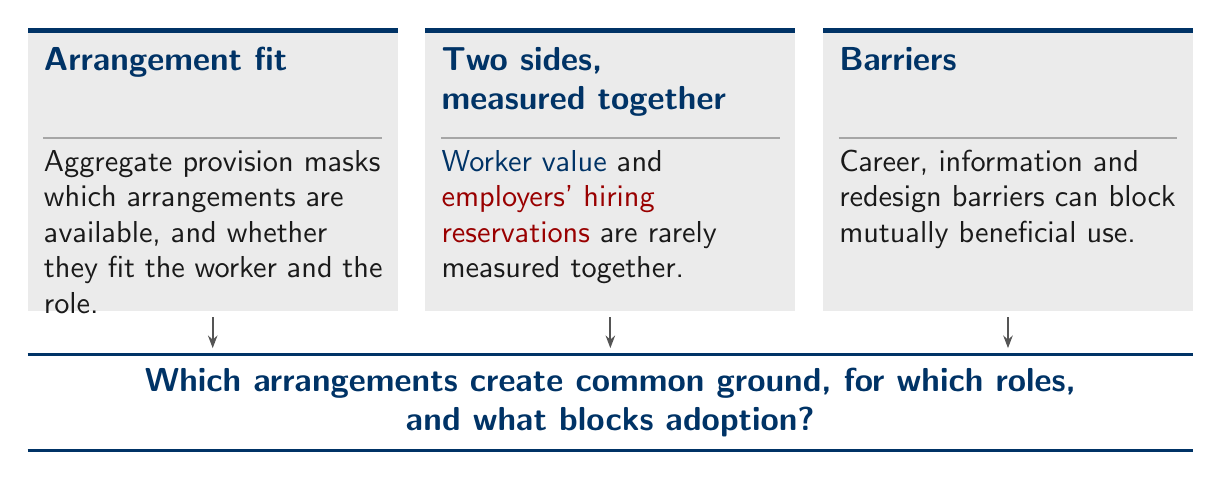
\begin{tikzpicture}[x=1cm,y=1cm,trim left=0cm,trim right=14.8cm] % trim: the 0.8 pt navy rules end on the margins
    % card 1: arrangement fit
    \DeckCard{0}{0}{4.7}{-3.60}{Navy}
    \node[deckhead=Navy] at (0.2,-0.25) {Arrangement fit};
    \draw[Rule,line width=0.6pt] (0.2,-1.40) -- (4.5,-1.40);
    \node[deckbody,text width=4.3cm] at (0.2,-1.55) {Aggregate provision masks which arrangements are available, and whether they fit the worker and the role.};
    % card 2: the two sides are rarely measured together. Fixer pass 7 Oct 2026 (mom_ps-03, editor-02): the spec's
    % wording, have not been measured together, is contradicted by the deck's own M-literature row 2 [R16, L1]
    \DeckCard{5.05}{0}{9.75}{-3.60}{Navy}
    \node[deckhead=Navy] at (5.25,-0.25) {Two sides,\\measured together};
    \draw[Rule,line width=0.6pt] (5.25,-1.40) -- (9.55,-1.40);
    \node[deckbody,text width=4.3cm] at (5.25,-1.55) {\textcolor{Employee}{Worker value} and \textcolor{Employer}{employers' hiring reservations} are rarely measured together.};
    % card 3: barriers
    \DeckCard{10.10}{0}{14.80}{-3.60}{Navy}
    \node[deckhead=Navy] at (10.30,-0.25) {Barriers};
    \draw[Rule,line width=0.6pt] (10.30,-1.40) -- (14.60,-1.40);
    \node[deckbody,text width=4.3cm] at (10.30,-1.55) {Career, information and redesign barriers can block mutually beneficial use.};
    % the connecting question
    \draw[deckarrow] (2.35,-3.68) -- (2.35,-4.07);
    \draw[deckarrow] (7.40,-3.68) -- (7.40,-4.07);
    \draw[deckarrow] (12.45,-3.68) -- (12.45,-4.07);
    \draw[Navy,line width=0.8pt] (0,-4.15) -- (14.8,-4.15);
    \node[anchor=center,text width=14.4cm,align=center,inner sep=0pt,font=\FsHead,text=Navy] at (7.4,-4.76)
      {Which arrangements create common ground, for which roles,\\and what blocks adoption?};
    \draw[Navy,line width=0.8pt] (0,-5.37) -- (14.8,-5.37);
  \end{tikzpicture}\par
  \Backups{\BL{B-guidelines}{Guidelines} \BL{B-partners}{Partners}}
\end{frame}
% Note numbers: none spoken. Context only: [P1] the Guidelines set a process; [P2] no administrative request counts;
% [P3] MOM's need-request data, almost entirely pre-Guidelines, and MOM's frictions reading (spoken, no number; mom_ps-03);
% [D9, B6] our request item was partly misread and no why-not item exists; [R16, L1] the Polish two-sided study
\note{[Short path] The Guidelines already set a process for requests. MOM's own survey finds that few who need an arrangement ask formally, a gap MOM attributes to frictions rather than employer resistance. % [P3]
What remains open is fit, in three parts.
First, high overall provision can hide which arrangements are on offer, and whether they suit the worker and the role.
Second, few studies measure together how workers value each arrangement and how employers weigh it in hiring; a Polish study is one. % [R16, L1]
Third, career worries, unclear terms and the effort of job redesign can block arrangements that would suit both sides; reasons for not asking are rarely measured.
For the partners, the question is which arrangements to make easier to try now, which to tailor by role, which to test before scaling, and what information is missing.
We use a simple map. [Full deck: first, where this sits in the research.]}

% ==========================================================================
% 4. RELATED LITERATURE AND CONTRIBUTION   [full deck only]
% ==========================================================================
% Directive 4: three rows, bold row labels in their own column, a thin rule between every row, and the same
% three fields in every row; no Takeaway; citations in the one-line source note.
% Polish pass, 7 Oct 2026 (DESIGN_PLAN s2 W1, G8): the shared \MainTableStyle; columns 2.6 / 2.8 / X / 3.0 cm;
% bottom-aligned bold headers via \HeadB; row labels bold Ink; the note is labelled References and breaks after
% the third citation into two balanced lines. Adapted: the type is \FsTableTight, 9.5 pt, the pre-polish size,
% not \FsTable 10 pt. At 10 pt the table plus the two-line References note left 0.05 cm of slack, below the
% 0.10 cm floor, with the note touching the bottom rule; at 9.5 pt the slack is at least 0.30 cm.
\begin{frame}[t,label=M-literature]{Two-sided evidence remains limited}
  % Row 1: [E16, L1] WFH option about 4-8% of pay, the team's span of four headline estimates, designs differ;
  %        Aksoy et al. Singapore 4.8%, one online wave in early 2022, about 90% tertiary-educated [L1, E16]
  % Row 2: [R16, L1] IZA DP 16041, 2023 working paper: workers 2.9%, employers 21%, hybrid and fully remote pooled;
  %        [P7, L1] six-month hybrid RCT, quits cut by one-third
  % Row 3: [P4s] MRSD provision series; [L1] Wang and Dong 2024, vignette experiment
  % Column 3: [S7] seven arrangement levels; [S5] mirrored hiring task; [S1, S2, P1] fielded Aug-Oct 2026, after 1 Dec 2024
  \FrameTop % first body token (centring; never a frame subtitle)
  {\MainTableStyle\FsTableTight
  \begin{tabularx}{\linewidth}{@{}>{\raggedright\arraybackslash}p{2.6cm}>{\raggedright\arraybackslash}p{2.8cm}>{\raggedright\arraybackslash}X>{\raggedright\arraybackslash}p{3.0cm}@{}}
    \toprule
    & \HeadB{\linewidth}{What existing work measures} & \HeadB{\linewidth}{What it finds \mdseries(not like-for-like)} & \HeadB{\linewidth}{What this study adds}\\
    \midrule
    \textbf{Worker value of WFH}
      & Pay workers would give up for a WFH option
      & About 4--8\% of pay; Singapore 4.8\%, in an online, mostly tertiary-educated sample % [E16, L1]
      & Seven arrangements, one design\\ % [S7]
    \midrule
    \textbf{Employer side and productivity}
      & Employers' expected costs; quits in a firm trial
      & Poland (2023 working paper, hybrid and remote pooled): workers give up 2.9\%, employers expect a 21\% wage cut. Hybrid trial: quits fell by a third % [R16, P7, L1]
      & Employers' hiring choices, mirrored with PMEs'\\ % [S5]
    \midrule
    \textbf{Singapore}
      & Which firms offer FWAs; stated intentions
      & Provision is widespread; FWAs raise stated fertility intentions % [P4s, L1]
      & Both sides' choices, after the Guidelines took effect\\ % [S1, S2, P1]
    \bottomrule
  \end{tabularx}\par}
  \SourceNote{\textbf{References:} Mas \& Pallais 2017; Maestas et al.\ 2023; Aksoy et al.\ 2022;\\ Lewandowski et al.\ 2023; Bloom et al.\ 2024; MRSD; Wang \& Dong 2024.} % [L1, R16, P7, P4s]
  \Backups{\BL{B-emp-benchmarks}{Benchmarks} \BL{B-intl}{Trials}}
\end{frame}
% Note numbers: [E16, L1] 4 to 8, 27 countries, 4.8; [R16] about 3 from 2.9, 21, gap mostly expected productivity loss, published 5.2 and 24.6; [P7] six-month trial, a third
\note{[Full deck only] Three strands frame the study. First, worker valuations: abroad, a work-from-home option is worth about 4 to 8 per cent of pay; a 27-country survey puts Singapore at 4.8 per cent, from an online, mostly tertiary-educated sample. % [E16, L1]
Second, the employer side: a 2023 Polish working paper finds workers give up about 3 per cent of pay for remote or hybrid work, while employers expect a 21 per cent wage cut, mostly from expected productivity loss. A six-month trial found hybrid work cut quits by a third. % [R16, P7]
[If asked: the published version, ILR Review 2026, reports gaps of about 5 per cent of earnings for hybrid and 25 per cent for fully remote work.] % [R16] 5.2 and 24.6
Third, Singapore evidence is mostly descriptive. Our study complements this work by observing both sides on a common menu.
Next, a simple map for reading the results.}

% ==========================================================================
% 5. CONCEPTUAL FRAMEWORK   [short path]
% ==========================================================================
% Directive 5: three large horizontal zone cards and a barrier strip; no algebra and no axes. A conceptual map:
% no data and no numbers. PMEs in myblue, employers in myred, zone cards neutral grey.
% Geometry (polish pass, 7 Oct 2026; DESIGN_PLAN s2 W1, G7): column heads to y = +0.41; full-row Soft bands
% 1.45 cm tall, 0.15 cm apart, y = 0 to -4.65, the same band grammar as M-discussion; barrier strip y = -4.95 to
% -5.65; the picture is 6.06 cm tall. Shared styles: deckdisc, deckcolhead, deckarrow, type scale FsHead/FsBody.
\begin{frame}[t,label=M-framework]{Three zones, three policy moves}
  \FrameTop % polish pass: replaces the 0.15 cm vspace
  \noindent
  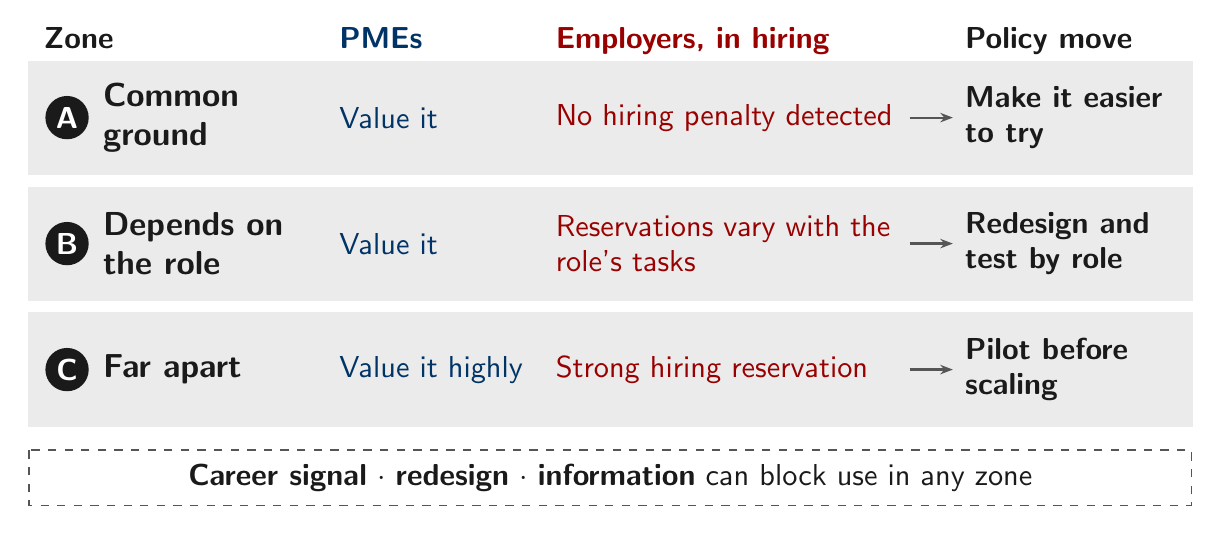
\begin{tikzpicture}[x=1cm,y=1cm,
      band/.style={deckcard},
      zl/.style={deckdisc},
      zn/.style={anchor=west,text width=2.75cm,align=left,inner sep=0pt,font=\FsHead,text=Ink},
      pm/.style={anchor=west,text width=2.6cm,align=left,inner sep=0pt,font=\FsBody,text=Employee},
      em/.style={anchor=west,text width=4.4cm,align=left,inner sep=0pt,font=\FsBody,text=Employer},
      mv/.style={anchor=west,text width=2.8cm,align=left,inner sep=0pt,font=\FsBody\bfseries,text=Ink},
      hdr/.style={deckcolhead},
      arr/.style={deckarrow}]
    % column heads (polish pass: all bold \FsBody; Zone and Policy move in Ink, the two sides in their colours)
    \node[hdr,text=Ink] at (0.20,0.15) {Zone};
    \node[hdr,text=Employee] at (3.95,0.15) {PMEs};
    \node[hdr,text=Employer] at (6.70,0.15) {Employers, in hiring};
    \node[hdr,text=Ink] at (11.90,0.15) {Policy move};
    % A: common ground
    \fill[band] (0,0) rectangle (14.8,-1.45);
    \node[zl] at (0.50,-0.725) {A};
    \node[zn] at (0.95,-0.725) {Common\\ground};
    \node[pm] at (3.95,-0.725) {Value it};
    \node[em] at (6.70,-0.725) {No hiring penalty detected};
    \draw[arr] (11.20,-0.725) -- (11.75,-0.725);
    \node[mv] at (11.90,-0.725) {Make it easier\\to try};
    % B: depends on the role
    \fill[band] (0,-1.60) rectangle (14.8,-3.05);
    \node[zl] at (0.50,-2.325) {B};
    \node[zn] at (0.95,-2.325) {Depends on\\the role};
    \node[pm] at (3.95,-2.325) {Value it};
    \node[em] at (6.70,-2.325) {Reservations vary with the role's tasks};
    \draw[arr] (11.20,-2.325) -- (11.75,-2.325);
    \node[mv] at (11.90,-2.325) {Redesign and\\test by role};
    % C: far apart
    \fill[band] (0,-3.20) rectangle (14.8,-4.65);
    \node[zl] at (0.50,-3.925) {C};
    \node[zn] at (0.95,-3.925) {Far apart};
    \node[pm] at (3.95,-3.925) {Value it highly};
    \node[em] at (6.70,-3.925) {Strong hiring reservation};
    \draw[arr] (11.20,-3.925) -- (11.75,-3.925);
    \node[mv] at (11.90,-3.925) {Pilot before\\scaling};
    % barriers, in any zone
    \draw[Muted,dashed,line width=0.6pt] (0.02,-4.95) rectangle (14.78,-5.65);
    \node[anchor=center,inner sep=0pt,font=\FsBody,text=Ink] at (7.40,-5.30)
      {\textbf{Career signal} $\cdot$ \textbf{redesign} $\cdot$ \textbf{information} can block use in any zone};
  \end{tikzpicture}\par
  \Backups{\BL{B-methods}{Methods} \BL{B-intl}{Trials}}
\end{frame}
% Note numbers: none. Information problem per MANDATE: a hiring reservation may reflect operating constraints,
% uncertainty or a candidate signal, and the hiring choices cannot separate them [S5; B-limits]
\note{[Short path] We read every result on this map. For each arrangement, we ask how much PMEs value it, and how strongly employers hold back when hiring someone who wants it.
Where PMEs value it and we detect no hiring penalty, there is common ground: firms and SNEF could make it easier to try.
Where reservations depend on the role's tasks, firms can redesign jobs and test role by role.
Where PMEs value it highly but employers hold strong reservations, the sides are far apart: pilot with volunteer firms before scaling.
A reservation may reflect real operating constraints, uncertainty, or what a request seems to signal; hiring choices cannot separate these; a pilot can show whether operating constraints materialise.
In any zone, career signals, redesign and missing information can block use.
Next, how we asked both sides. [Full deck: next, the two surveys.]}

% ##########################################################################
% Main slides from redesign/v3/W2_frames.tex
% ##########################################################################
\begin{frame}[t,label=M-data]{Two surveys, unweighted online panels}
  \FrameTop
  \FigC{F_sample_m}
  % [S1, S2, S4] unweighted online panels: shares describe the surveyed samples only
  \Interp{Shares describe surveyed PMEs and firms, not national rates.}
  % [S1] PME survey fielded 4-21 Aug 2026; [S2] employer survey 12 Aug-2 Oct 2026
  \SourceNote{\textbf{Source:} this study's PME survey (Aug 2026) and employer survey (Aug--Oct 2026).}
  \Backups{\BL{B-sample}{Sample}\BL{B-panel}{Panels}}
\end{frame}
% note facts: [S1] 1,020, 4-21 Aug 2026; [S2] 397 (appended sample), 12 Aug-2 Oct 2026; [S1, S2, S4] online, unweighted;
% [S3] 12%, about one firm in eight; [F2] the employer survey asked no re-contact question, so firm-side work
% needs fresh volunteers
% implication, spoken: shares describe the samples; SNEF could help recruit smaller firms, as fresh volunteers
\note{[Full deck only]
We surveyed both sides of the same labour market.
1,020 citizens and permanent residents in or seeking PME roles answered between 4 and 21 August 2026; % [S1]
397 people involved in PME hiring or manpower decisions answered between 12 August and 2 October. % [S2]
Both samples come from unweighted online panels, so our shares describe the PMEs and firms we surveyed: MOM's surveys give national rates; ours give the trade-offs. % [S1, S2, S4]
We acknowledge that the employer sample leans large: only \Pend{about one firm in eight} has 50 or fewer staff. % [S3] not in appended_* outputs
SNEF could help recruit smaller member firms, as fresh volunteers, for any next round. % [F2]
Next, the choice task.}

% ==========================================================================
% 7. DESIGN   [short path]
% ==========================================================================
% One large mirrored choice card on a common FWA menu (COMMENTS slide 7; ROUND5_SPEC s3 row 7).
% PME columns (myblue) and employer columns (myred) share the attribute spine in the middle.
% Example pair, illustrative: A = reference pay x 1.10, fully onsite, fixed hours; B = x 0.90, 1-2 WFH days,
% compressed 4-day week [S6b: 0.90/1.10 was drawn; gap 18%, inside 17-33%, S6]; levels [S7]; the rest is
% held at the respondent's own practice [S5]. Reference pay: own salary (PMEs), the firm's most recent PME
% hire (employers) [S6]. Sample facts from M-data moved here (COMMENTS slide 6): [S1] [S2] [S3]. [S2] now 397 (appended).
\begin{frame}[t,label=M-design]{Mirrored choices on a common FWA menu}
  \FrameTop % first body token (centring; never a frame subtitle)
  {\centering
  % Polish pass (DESIGN_PLAN s2, W2): shared deck styles; column heads are coloured bold text over a
  % 1.2 pt rule in the side colour (no text on a dark fill); cells deckcell, held boxes deckheld, chips deckchip.
  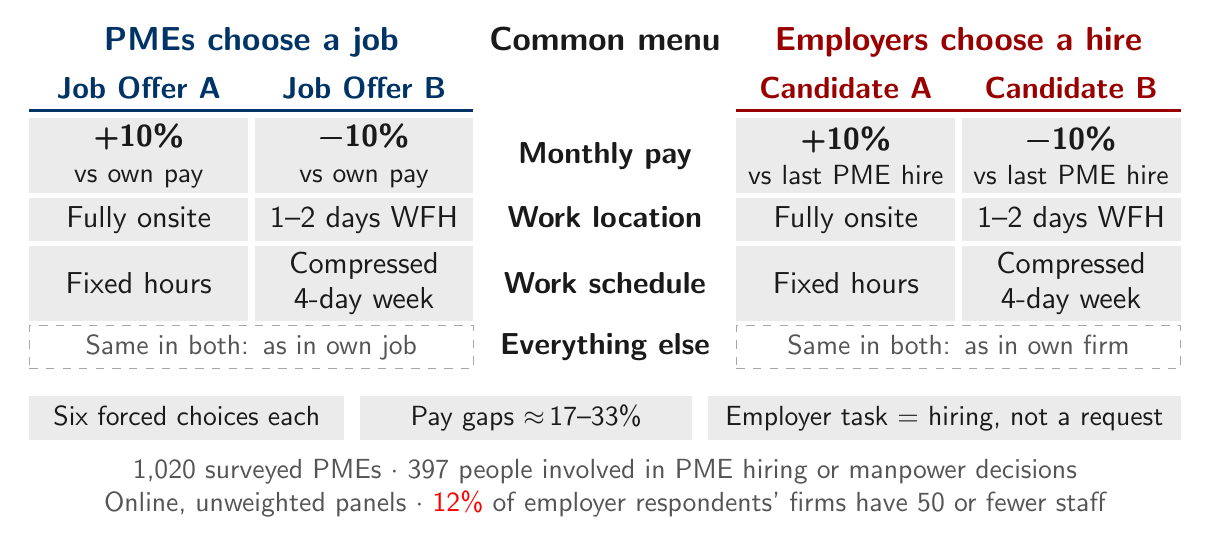
\begin{tikzpicture}[x=1cm,y=1cm,every node/.style={outer sep=0pt},
      hd/.style={anchor=base,inner sep=0pt,font=\FsHead},
      ch/.style={anchor=base west,inner xsep=0.08cm,inner ysep=0pt,minimum width=2.78cm,
        text width=2.62cm,align=center,font=\FsBody\bfseries},
      one/.style={text height=0.27cm,text depth=0.08cm},
      cell/.style={deckcell,anchor=north west,minimum width=2.78cm,text width=2.62cm},
      lab/.style={anchor=north,inner xsep=0.04cm,inner ysep=0.03cm,minimum width=3.18cm,align=center,text=Ink,
        font=\FsBody\bfseries},
      same/.style={deckheld,anchor=north west,inner xsep=0.08cm,inner ysep=0.03cm,minimum width=5.64cm,
        text width=5.48cm,minimum height=0.55cm},
      chip/.style={deckchip,anchor=north west,inner ysep=0.03cm}]
    % ---- side headers (common baseline y = -0.36)
    \node[hd,text=Employee,minimum width=5.64cm] at (2.82,-0.36) {PMEs choose a job};
    \node[hd,text=Ink,minimum width=3.18cm] at (7.31,-0.36) {Common menu};
    \node[hd,text=Employer,minimum width=5.64cm] at (11.80,-0.36) {Employers choose a hire};
    % ---- column heads (instrument labels: Job Offer A/B; Candidate A/B) on baseline y = -0.97, with a rule
    % under each pair
    \node[ch,text=Employee] at (0,-0.97) {Job Offer A};
    \node[ch,text=Employee] at (2.86,-0.97) {Job Offer B};
    \node[ch,text=Employer] at (8.98,-0.97) {Candidate A};
    \node[ch,text=Employer] at (11.84,-0.97) {Candidate B};
    \draw[Employee,line width=1.2pt] (0,-1.12) -- (5.64,-1.12);
    \draw[Employer,line width=1.2pt] (8.98,-1.12) -- (14.62,-1.12);
    % ---- pay row: [S6b] multipliers 1.10 and 0.90 = 10% above and below the reference pay [S6]
    \node[cell,minimum height=0.95cm] at (0,-1.22) {\textbf{+10\%}\\{\FsSmall vs own pay}};
    \node[cell,minimum height=0.95cm] at (2.86,-1.22) {\textbf{\textminus 10\%}\\{\FsSmall vs own pay}};
    \node[lab,minimum height=0.95cm] at (7.31,-1.22) {Monthly pay};
    \node[cell,minimum height=0.95cm] at (8.98,-1.22) {\textbf{+10\%}\\{\FsSmall vs last PME hire}};
    \node[cell,minimum height=0.95cm] at (11.84,-1.22) {\textbf{\textminus 10\%}\\{\FsSmall vs last PME hire}};
    % ---- location row: levels [S7]
    \node[cell,one,minimum height=0.55cm] at (0,-2.23) {Fully onsite};
    \node[cell,one,minimum height=0.55cm] at (2.86,-2.23) {1--2 days WFH};
    \node[lab,one,minimum height=0.55cm] at (7.31,-2.23) {Work location};
    \node[cell,one,minimum height=0.55cm] at (8.98,-2.23) {Fully onsite};
    \node[cell,one,minimum height=0.55cm] at (11.84,-2.23) {1--2 days WFH};
    % ---- schedule row: levels [S7]; compressed 4-day week = same total hours over four longer days [S7]
    \node[cell,minimum height=0.95cm] at (0,-2.84) {Fixed hours};
    \node[cell,minimum height=0.95cm] at (2.86,-2.84) {Compressed\\4-day week};
    \node[lab,minimum height=0.95cm] at (7.31,-2.84) {Work schedule};
    \node[cell,minimum height=0.95cm] at (8.98,-2.84) {Fixed hours};
    \node[cell,minimum height=0.95cm] at (11.84,-2.84) {Compressed\\4-day week};
    % ---- held row: [S5] all other attributes at the respondent's own current practice, both sides
    \node[same,one] at (0,-3.85) {Same in both: as in own job};
    \node[lab,one,minimum height=0.55cm] at (7.31,-3.85) {Everything else};
    \node[same,one] at (8.98,-3.85) {Same in both: as in own firm};
    % ---- three guardrails, 0.2 cm apart, spanning the card width: [S5] six forced choices; [S6, S6b] pay gaps
    % 17-33% by design (displayed about 16-34% after S$50 rounding, S6; fixer pass 7 Oct 2026, editor-13: the
    % spec chip wording, without always); [S5; EB s9; Lead decision 7] the employer task is a hire, not a reply
    % to a request
    \node[chip,one,minimum width=4.00cm,text width=3.76cm] at (0,-4.75) {Six forced choices each};
    \node[chip,one,minimum width=4.22cm,text width=3.98cm] at (4.20,-4.75) {Pay gaps \ap 17--33\%};
    \node[chip,one,minimum width=6.00cm,text width=5.76cm] at (8.62,-4.75) {Employer task = hiring, not a request};
    % ---- sample: [S1] 1,020 PMEs; [S2] 397 people involved in PME hiring or manpower decisions;
    % [S1, S2, S4] online panels, unweighted; [S3] 12% of employer respondents' firms have 50 or fewer staff
    \node[anchor=north,inner sep=0pt,text width=14.6cm,align=center,text=Muted,font=\FsSmall]
      at (7.31,-5.55) {1,020 surveyed PMEs $\cdot$ 397 people involved in PME hiring or manpower decisions\\ % [S1, S2]; 397 = appended sample
      Online, unweighted panels $\cdot$ \Pend{12\%} of employer respondents' firms have 50 or fewer staff}; % [S3, S4]; S3 not in appended_* outputs
  \end{tikzpicture}\par}
  \Backups{\BL{B-cards}{Choice cards}\BL{B-sample}{Sample}}
\end{frame}
% note facts: [S1] 1,020; [S2] 397; [S1, S2, S4] online, unweighted; [S3] firms lean large; [S5] six choices,
% two options, the rest held at own practice; [S6b] 10% above / below = multipliers 1.10 / 0.90; [S7] compressed
% week = same total hours over four longer days; [S6] 17 to 33 per cent; EB s9 and Lead decision 7: a hire,
% not a reply to a request; EB s3b and s9: magnitudes are model-based, so rankings are firmer than prices
% implication, spoken: partners get an arrangement-by-arrangement reading of each side, not one offer rate
\note{[Short path]
Both sides chose from one FWA menu.
We surveyed 1,020 PMEs and 397 people involved in PME hiring or manpower decisions, from unweighted online panels; the firms lean large. % [S1, S2, S3, S4]
Each PME chose six times between two job offers; each employer, between two equally qualified candidates. % [S5]
Here, offer A pays 10 per cent above the PME's own pay and B 10 per cent below, but B has one to two WFH days and a compressed week: the same hours over four longer days. % [S6b, S7]
Pay gaps were 17 to 33 per cent by design, so rankings are firmer than prices. % [S6, EB s9]
For employers, this is a hiring choice, not a reply to a request. % [S5; EB s9]
Now the results, starting with PMEs. [Full deck: ``Next, how we turn these choices into values.'']}

